% Тип документа
\documentclass[a4paper,12pt]{extarticle}

% Шрифты, кодировки, символьные таблицы, переносы
\usepackage{cmap}
\usepackage[T2A]{fontenc}
\usepackage[utf8x]{inputenc}
\usepackage[russian]{babel}

% Это пакет -- хитрый пакет, он нужен но не нужен
\usepackage[mode=buildnew]{standalone}

\usepackage
	{
		% Дополнения Американского математического общества (AMS)
		amssymb,
		amsfonts,
		amsmath,
		amsthm,
		physics,
		% misccorr,
		% 
		% Графики и рисунки
		wrapfig,
		graphicx,
		subcaption,
		float,
		tikz,
		tikz-3dplot,
		caption,
		csvsimple,
		color,
		booktabs,
		pgfplots,
		pgfplotstable,
		geometry,
		% 
		% Таблицы, списки
		array,
		makecell,
		multirow,
		indentfirst,
		%
		% Интегралы и прочие обозначения
		ulem,
		esint,
		esdiff,
		% 
		% Колонтитулы
		fancyhdr,
	}  

\usepackage{xcolor}
\usepackage{hyperref}

 % Цвета для гиперссылок
\definecolor{linkcolor}{HTML}{000000} % цвет ссылок
\definecolor{urlcolor}{HTML}{799B03} % цвет гиперссылок
 
\hypersetup{pdfstartview=FitH,  linkcolor=linkcolor,urlcolor=urlcolor, colorlinks=true}
% Обводка текста в TikZ
\usepackage[outline]{contour}

% Увеличенный межстрочный интервал, французские пробелы
\linespread{1.3} 
\frenchspacing 

 
\usetikzlibrary
	{
		decorations.pathreplacing,
		decorations.pathmorphing,
		patterns,
		calc,
		scopes,
		arrows,
		fadings,
		through,
		shapes.misc,
		arrows.meta,
		3d,
		quotes,
		angles,
		babel
	}


\tikzset{
	force/.style=	{
		>=latex,
		draw=blue,
		fill=blue,
				 	}, 
	%				 	
	axis/.style=	{
		densely dashed,
		blue,
		line width=1pt,
		font=\small,
					},
	%
	th/.style=	{
		line width=1pt},
	%
	acceleration/.style={
		>=open triangle 60,
		draw=magenta,
		fill=magenta,
					},
	%
	inforce/.style=	{
		force,
		double equal sign distance=2pt,
					},
	%
	interface/.style={
		pattern = north east lines, 
		draw    = none, 
		pattern color=gray!60,
					},
	cross/.style=	{
		cross out, 
		draw=black, 
		minimum size=2*(#1-\pgflinewidth), 
		inner sep=0pt, outer sep=0pt,
					},
	%
	cargo/.style=	{
		rectangle, 
		fill=black!70, 
		inner sep=2.5mm,
					},
	%
	caption/.style= {
		midway,
		fill=white!20, 
		opacity=0.9
					},
	%
	}

\newenvironment{tikzpict}
    {
	    \begin{figure}[htbp]
		\centering
		\begin{tikzpicture}
    }
    { 
		\end{tikzpicture}
		% \caption{caption}
		% \label{fig:label}
		\end{figure}
    }


\newcommand{\vbLabel}[3]{\draw ($(#1,#2)+(0,5pt)$) -- ($(#1,#2)-(0,5pt)$) node[below]{#3}}
\newcommand{\vaLabel}[3]{\draw ($(#1,#2)+(0,5pt)$) node[above]{#3} -- ($(#1,#2)-(0,5pt)$) }

\newcommand{\hrLabel}[3]{\draw ($(#1,#2)+(5pt,0)$) -- ($(#1,#2)-(5pt,0)$) node[right, xshift=1em]{#3}}
\newcommand{\hlLabel}[3]{\draw ($(#1,#2)+(5pt,0)$) node[left, xshift=-1em]{#3} -- ($(#1,#2)-(5pt,0)$) }



\newcommand\zi{^{\,*}_i}
\newcommand\sumn{\sum_{i=1}^{N}}

\tikzset{
	coordsys/.style={scale=1.8,x={(1.1cm,-0cm)},y={(0.5cm,1cm)}, z={(0cm,0.8cm)}},
	coordsys/.style={scale=1.5,x={(0cm,0cm)},y={(1cm,0cm)}, z={(0cm,1cm)}}, 
	coordsys/.style={scale=1.5,x={(1cm,0cm)},y={(0cm,1cm)}, z={(0cm,0cm)}}, 
}

\usepgfplotslibrary{units}


% Draw line annotation
% Input:
%   #1 Line offset (optional)
%   #2 Line angle
%   #3 Line length
%   #5 Line label
% Example:
%   \lineann[1]{30}{2}{$L_1$}

\newcommand{\lineann}[4][0.5]{%
    \begin{scope}[rotate=#2, blue,inner sep=2pt, ]
        \draw[dashed, blue!40] (0,0) -- +(0,#1)
            node [coordinate, near end] (a) {};
        \draw[dashed, blue!40] (#3,0) -- +(0,#1)
            node [coordinate, near end] (b) {};
        \draw[|<->|] (a) -- node[fill=white, scale=0.8] {#4} (b);
    \end{scope}
}

\newcommand{\lineannn}[4][0.5]{%
    \begin{scope}[rotate=#2, blue,inner sep=2pt, ]
        \draw[dashed, blue!40] (0,0) -- +(0,#1)
            node [coordinate, near end] (a) {};
        \draw[dashed, blue!40] (#3,0) -- +(0,#1)
            node [coordinate, near end] (b) {};
        % \draw[color=white, color=blue] (a) -- node[fill=white, scale=0.8] {#4} (b);
        \draw[->|] (a)++(-0.3,0) -- (a);
        \draw[->|] (b)++(0.3,0) coordinate (xx) -- (b);
        \draw (xx) node[fill=white, scale=0.8, right] {#4};
    \end{scope}
}

% Круговая стрелка относительно центра (дуга из центра)
\tikzset{
  pics/carc/.style args={#1:#2:#3}{
    code={
      \draw[pic actions] (#1:#3) arc(#1:#2:#3);
    }
  },
  dash/.style={
  	dash pattern=on 5mm off 5mm
  }
}

% Среднее <#1>
\newcommand{\mean}[1]{\langle#1\rangle}

\pgfplotsset{
    % most recent feature set of pgfplots
    compat=newest,
}

% const прямым шрифтом
\newcommand\ct[1]{\text{\rmfamily\upshape #1}}
\newcommand*{\const}{\ct{const}}


\usepackage[europeanresistors,americaninductors]{circuitikz}

% Style to select only points from #1 to #2 (inclusive)
\pgfplotsset{select/.style 2 args={
    x filter/.code={
        \ifnum\coordindex<#1\def\pgfmathresult{}\fi
        \ifnum\coordindex>#2\def\pgfmathresult{}\fi
    }
}}


\usepackage{array}
\usepackage{pstool}


%%%%%%%%%%%%%%%%%%%%%%%%%%%%%%%%%%%%%%%%%%%%%%%%%
\makeatletter
\newif\if@gather@prefix 
\preto\place@tag@gather{% 
  \if@gather@prefix\iftagsleft@ 
    \kern-\gdisplaywidth@ 
    \rlap{\gather@prefix}% 
    \kern\gdisplaywidth@ 
  \fi\fi 
} 
\appto\place@tag@gather{% 
  \if@gather@prefix\iftagsleft@\else 
    \kern-\displaywidth 
    \rlap{\gather@prefix}% 
    \kern\displaywidth 
  \fi\fi 
  \global\@gather@prefixfalse 
} 
\preto\place@tag{% 
  \if@gather@prefix\iftagsleft@ 
    \kern-\gdisplaywidth@ 
    \rlap{\gather@prefix}% 
    \kern\displaywidth@ 
  \fi\fi 
} 
\appto\place@tag{% 
  \if@gather@prefix\iftagsleft@\else 
    \kern-\displaywidth 
    \rlap{\gather@prefix}% 
    \kern\displaywidth 
  \fi\fi 
  \global\@gather@prefixfalse 
} 
\newcommand*{\beforetext}[1]{% 
  \ifmeasuring@\else
  \gdef\gather@prefix{#1}% 
  \global\@gather@prefixtrue 
  \fi
} 
\makeatother
%%%%%%%%%%%%%%%%%%%%%%%%%%%%%%%%%%%%%%%%%%%%%%%%%

\geometry		
	{
		left			=	2cm,
		right 			=	2cm,
		top 			=	3cm,
		bottom 			=	3cm,
		bindingoffset	=	0cm
	}

%%%%%%%%%%%%%%%%%%%%%%%%%%%%%%%%%%%%%%%%%%%%%%%%%%%%%%%%%%%%%%%%%%%%%%%%%%%%%%%



	%применим колонтитул к стилю страницы
\pagestyle{fancy} 
	%очистим "шапку" страницы
\fancyhead{} 
	%слева сверху на четных и справа на нечетных
\fancyhead[R]{\labauthors} 
	%справа сверху на четных и слева на нечетных
\fancyhead[L]{Отчёт по лабораторной работе №\labnumber} 
	%очистим "подвал" страницы
\fancyfoot{} 
	% номер страницы в нижнем колинтуле в центре
\fancyfoot[C]{\thepage} 

%%%%%%%%%%%%%%%%%%%%%%%%%%%%%%%%%%%%%%%%%%%%%%%%%%%%%%%%%%%%%%%%%%%%%%%%%%%%%%%

\renewcommand{\contentsname}{Оглавление}

\usepackage{tocloft}
% \renewcommand{\cftpartleader}{\cftdotfill{\cftdotsep}} % for parts
% \renewcommand{\cftsectiondotsep}{\cftdotsep}% Chapters should use dots in ToC
\renewcommand{\cftsecleader}{\cftdotfill{\cftdotsep}}
%\renewcommand{\cftsecleader}{\cftdotfill{\cftdotsep}} % for sections, if you really want! (It is default in report and book class (So you may not need it).
% ---------
% \newcommand{\cftchapaftersnum}{.}%
% \usepackage{titlesec}
% \titlelabel{\thetitle.\quad}
\usepackage{secdot}
\sectiondot{subsection}

\begin{document}

\def\labauthors{Виноградов И.Д., Шиков А.П.}
\def\labgroup{430}
\def\labnumber{5}
\def\labtheme{Опыт Франка-Герца}
\begin{titlepage}

\begin{center}

{\small\textsc{Нижегородский государственный университет имени Н.\,И. Лобачевского}}
\vskip 1pt \hrule \vskip 3pt
{\small\textsc{Радиофизический факультет}}

\vfill

{\Large Отчет по лабораторной работе №\labnumber\vskip 12pt\bfseries \labtheme}
	
\end{center}

\vfill
	
\begin{flushright}
	{Выполнили студенты \labgroup\ группы\\ \labauthors}%\vskip 12pt Принял:\\ Менсов С.\,Н.}
\end{flushright}
	
\vfill
	
\begin{center}
	Нижний Новгород, \the\year
\end{center}

\end{titlepage}



\section{Теоритическая часть}
{\bfseries Цель работы:} 
Экспериментально пронаблюдать дискретный характер поглощения энергии атомами, провести измерения потенциалов резонанса и
ионизации для атома гелия

На основании проведенных экспериментов Резерфордом в 1911 г. была построена планетарная модель атома. Но устойчивость такого атома и характер его спектров невозможно было объяснить с точки зрения известных тогда классической механики и электродинамики. Для устранения указанного противоречия Н. Бор в 1913 г. предложил квантовую теорию строения атома, в основе которой лежат следующие постулаты.


1.	Атомы могут длительно пребывать только в определенных энергетических состояниях. В этих состояниях они обладают энергиями $E_0,\,E_1,\,E_2\dots,\,E_n$, образующими дискретный ряд. При движении электронов по соответствующим этим состояниям стационарным орбитам никакого излучения или поглощения энергии не происходит.


2.	При переходе из одного энергетического состояния $E_m$, в другое $E_n$ поглощается или излучается строго определенная порция (квант) электромагнитной энергии. Энергия кванта связана с частотой излучения $\nu$ следующим отношением: $$h\nu=E_m-En,$$ где h - постоянная Планка.

Ставшие классическими эксперименты, выполненные в 1913 г. Д.Франком и Г. Герцем, непосредственно подтвердили справедливость квантовых постулатов Бора. В опыте Франка-Герца исследуются процессы столкновения электронов с атомами газа. Упрощенная схема экспериментальной установки приведена на рис.\ref{fig:1}. В баллоне лампы Д заполненной исследуемым газом, находятся три электрода: раскаленный катод К, являющийся источником электронов, сетка С и анод А. Между сеткой и катодом прикладывается разность потенциалов $\varphi_{y} =\varphi_{c} -\varphi_{k}$, ускоряющая электроны (потенциал сетки по отношению к катоду $\varphi_y$ называют ускоряющим потенциалом). Разность потенциалов между анодом и сеткой имеет, как правило, противоположный знак и носит название потенциала задержки $\varphi_{з} =\varphi_{a} -\varphi_{c}\textless{0}$.

\begin{center}
    \begin{minipage}[t]{0.49\linewidth}
        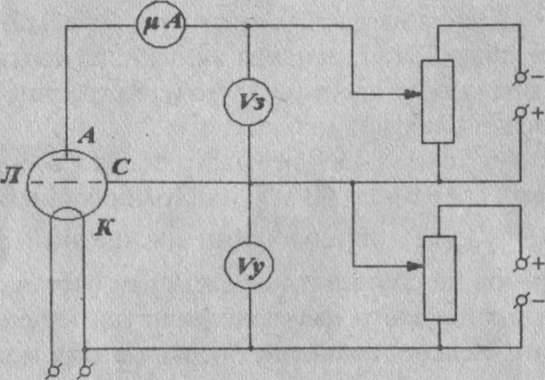
\includegraphics[width=\linewidth]{R1.png} 
        \label{fig:1}
        \vspace{-32pt}
        \captionof{figure}{} 
    \end{minipage}
    \begin{minipage}[t]{0.49\linewidth}
        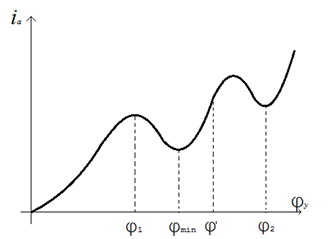
\includegraphics[width=\linewidth]{1.jpg} 
        \label{fig:2}
        \vspace{-32pt}
        \captionof{figure}{} 
    \end{minipage}
\end{center}

В ходе выполнения эксперимента снимается анодно-сеточная характеристика газонаполненной лампы, т. е. зависимость анодного 
тока $i_a$ от ускоряющего потенциала $\varphi_{y}$ при постоянном потенциале задержки $\varphi_{з}$. Типичный вид этой характеристики приведен на рис.2.

На начальном участке характеристики по мере увеличения $\varphi_y$ наблюдается монотонный рост анодного тока. В этом режиме вылетающие из катода электроны при движении к сетке приобретают сравнительно малую энергию $W_e$ и сталкиваются с атомами газа упруго. При таких столкновениях кинетическая энергия атома изменяется слабо - на величину порядка $$\Delta W\sim W_e\frac{m}{M}\ll W_e,$$ где m и M - массы электрона и атома соответственно, а внутреннее состояние атома не меняется. Поскольку при столкновениях атомы отбирают у электронов лишь незначительную часть энергии, последние, проходя через некоторую эквипотенциальную поверхность с потенциалом $\varphi$, имеют энергию, примерно равную $e\varphi$ (здесь не учтена начальная скорость вылета электронов с катода).

При $\varphi_{y} \textgreater \varphi_{з}$ электроны пролетают через сетку, имея энергию, достаточную для преодоления 
задерживающего потенциала, и достигают анода. Как и в обычных электронных лампах, с ростом потенциала сетки $\varphi_{y}$ анодный
 ток возрастает. Этот процесс продолжается до тех пор, пока $\varphi_{y}$ не достигнет величины
так называемого первого критического потенциала $\varphi_{1}$ (его называют также резонансным потенциалом), при котором электроны 
приобретают энергию, достаточную для возбуждения атома. Столкновения электронов, имеющих энергию $e\varphi_{1}$, с атомами могут 
происходить неупруго. При этом электрон в процессе столкновения всю свою энергию передает атому. Величина критического
потенциала $\varphi_{1}$ связана с разностью энергии возбужденного $E_1$, и невозбужденного $E_0$ атомов законом сохранения энергии: $$e\varphi_{1}=E_1-E_0.$$

Электроны, потерявшие энергию при неупругих столкновениях, не могут преодолеть задерживающего поля между анодом и сеткой
и <<вылавливаются>> последней, поэтому анодный ток с дальнейшим ростом $\varphi_{y}$ уменьшается. Так возникает падающий участок на анодно-сеточной характеристике.

При дальнейшем увеличении $\varphi_{y}$ поверхность с потенциалом $\varphi_{1}$ (а, следовательно, и область неупругих
соударений) смещается от сетки к катоду. При $\varphi_{y}\geqslant \varphi_{1}+|\varphi_{3}|$ электроны, испытавшие
неупругие соударения на пути к сетке, вновь могут набрать энергию, превышающую $e\varphi_{з}$, и анодный ток опять
возрастает с ростом $\varphi_{y}$. Начиная со значения $\varphi_{y}\geqslant2\varphi_{1}$, электроны на своем пути могут дважды неупруго столкнуться с атомами и, потеряв энергию после второго столкновения, не преодолеть задерживающий потенциал. Это приведет к появлению второго провала на анодно-сеточной характеристике. Аналогичным образом происходит падение тока и при более высоких потенциалах $\varphi_{n}=n\varphi_{1}$.


Заметим далее, что если на длине свободного пробега электрон может набрать энергию, большую разности энергий двух уровней $E_n-E_1$, то возможно возбуждение всех уровней с
энергией, меньшей $E_n$, и даже ионизация атома, если $E_n-E_1$ больше энергии ионизации. Поэтому уменьшение длины свободного пробега $\lambda$ (за счет увеличения давления газа внутри лампы) позволяет не только увеличить точность определения резонансного потенциала, но и избежать перекрытия различных ступеней возбуждения. С другой стороны, слишком сильное уменьшение $\lambda$ нецелесообразно, т. к. при этом электроны до прихода в область неупругих соударений $\Omega$ испытывают много упругих столкновений, что увеличивает их разброс по энергиям, и, следовательно, уменьшает точность определения резонансного потенциала.

Для некоторых газов, у которых величина резонансного потенциала не сильно отличается от потенциала ионизации, можно, используя эту же лампу, только при относительно больших потенциалах задержки ($\varphi_{3} /\varphi_{y} \sim1$), измерить также и потенциал ионизации.

Для этого можно использовать то обстоятельство, что при $|\varphi_{3}|\textgreater{\varphi_{y}}$, электроны, эмитированные катодом, не достигают анода, и анодный ток может быть вызван только положительными носителями заряда. В случае $|\varphi_{3}|\textgreater{\varphi_{y}}\geqslant{\varphi_{u}}$ наличие анодного тока связано с процессами ионизации электронным ударом в окрестностях сетки. Когда $\varphi_{y}$ достигнет значения $\varphi_{u}$, у витков сетки появится область неупругих соударений, в которой энергия электронов будет достаточна для ионизации атомов газа, и возникнет ионный ток между сеткой и анодом лампы. В анодной цепи ток в этом случае будет иметь направление, противоположное обычному и для его измерения необходимо произвести <<переполюсовку>> амперметра (заметим, что название <<анод>>\,в этом случае оказывается чисто условным).

Ранее утверждалось, что для точного определения резонансного потенциала необходимо избежать перекрытия различных ступеней возбуждения; а в этом случае электроны на длине свободного пробега должны набирать энергию, не превышающую разности уровней $\text{Е}_{2}-E_{1}$. Для ионизации же необходимо, чтобы энергия, полученная электроном на длине свободного пробега, была бы не меньше $E_{u}-E_1$ ($E_{u}$ - энергия, соответствующая ионизированному атому). Казалось бы, одновременное выполнение этих двух условий невозможно. Но нельзя забывать, что картины электрических полей внутри лампы при определении резонансного потенциала и потенциала ионизации будут совершенно различными. Нетрудно убедиться, что производная $\displaystyle\dv{\varphi}{n}$ во втором случае будет существенно выше, следовательно, и электрон в этом случае может набрать на длине свободного пробега существенно большую энергию $$\Delta W_{\lambda}=e\lambda \displaystyle\dv{\varphi}{n}.$$

\newpage
\section{Экспериментальная часть}

В Данной работе в качестве рабочего газа использовался гелий, при этом давление в лампе $\rho$=1.2 мм рт.ст.
\subsection{Определение резонансного уровня}
Напряжение накала $V_H$ = 3 В \\
Напряжение задержки $V_3$= 7.5 В \\
График зависимости анодного тока от ускоряющего потенциала:

\begin{minipage}{\linewidth}
    \centering
    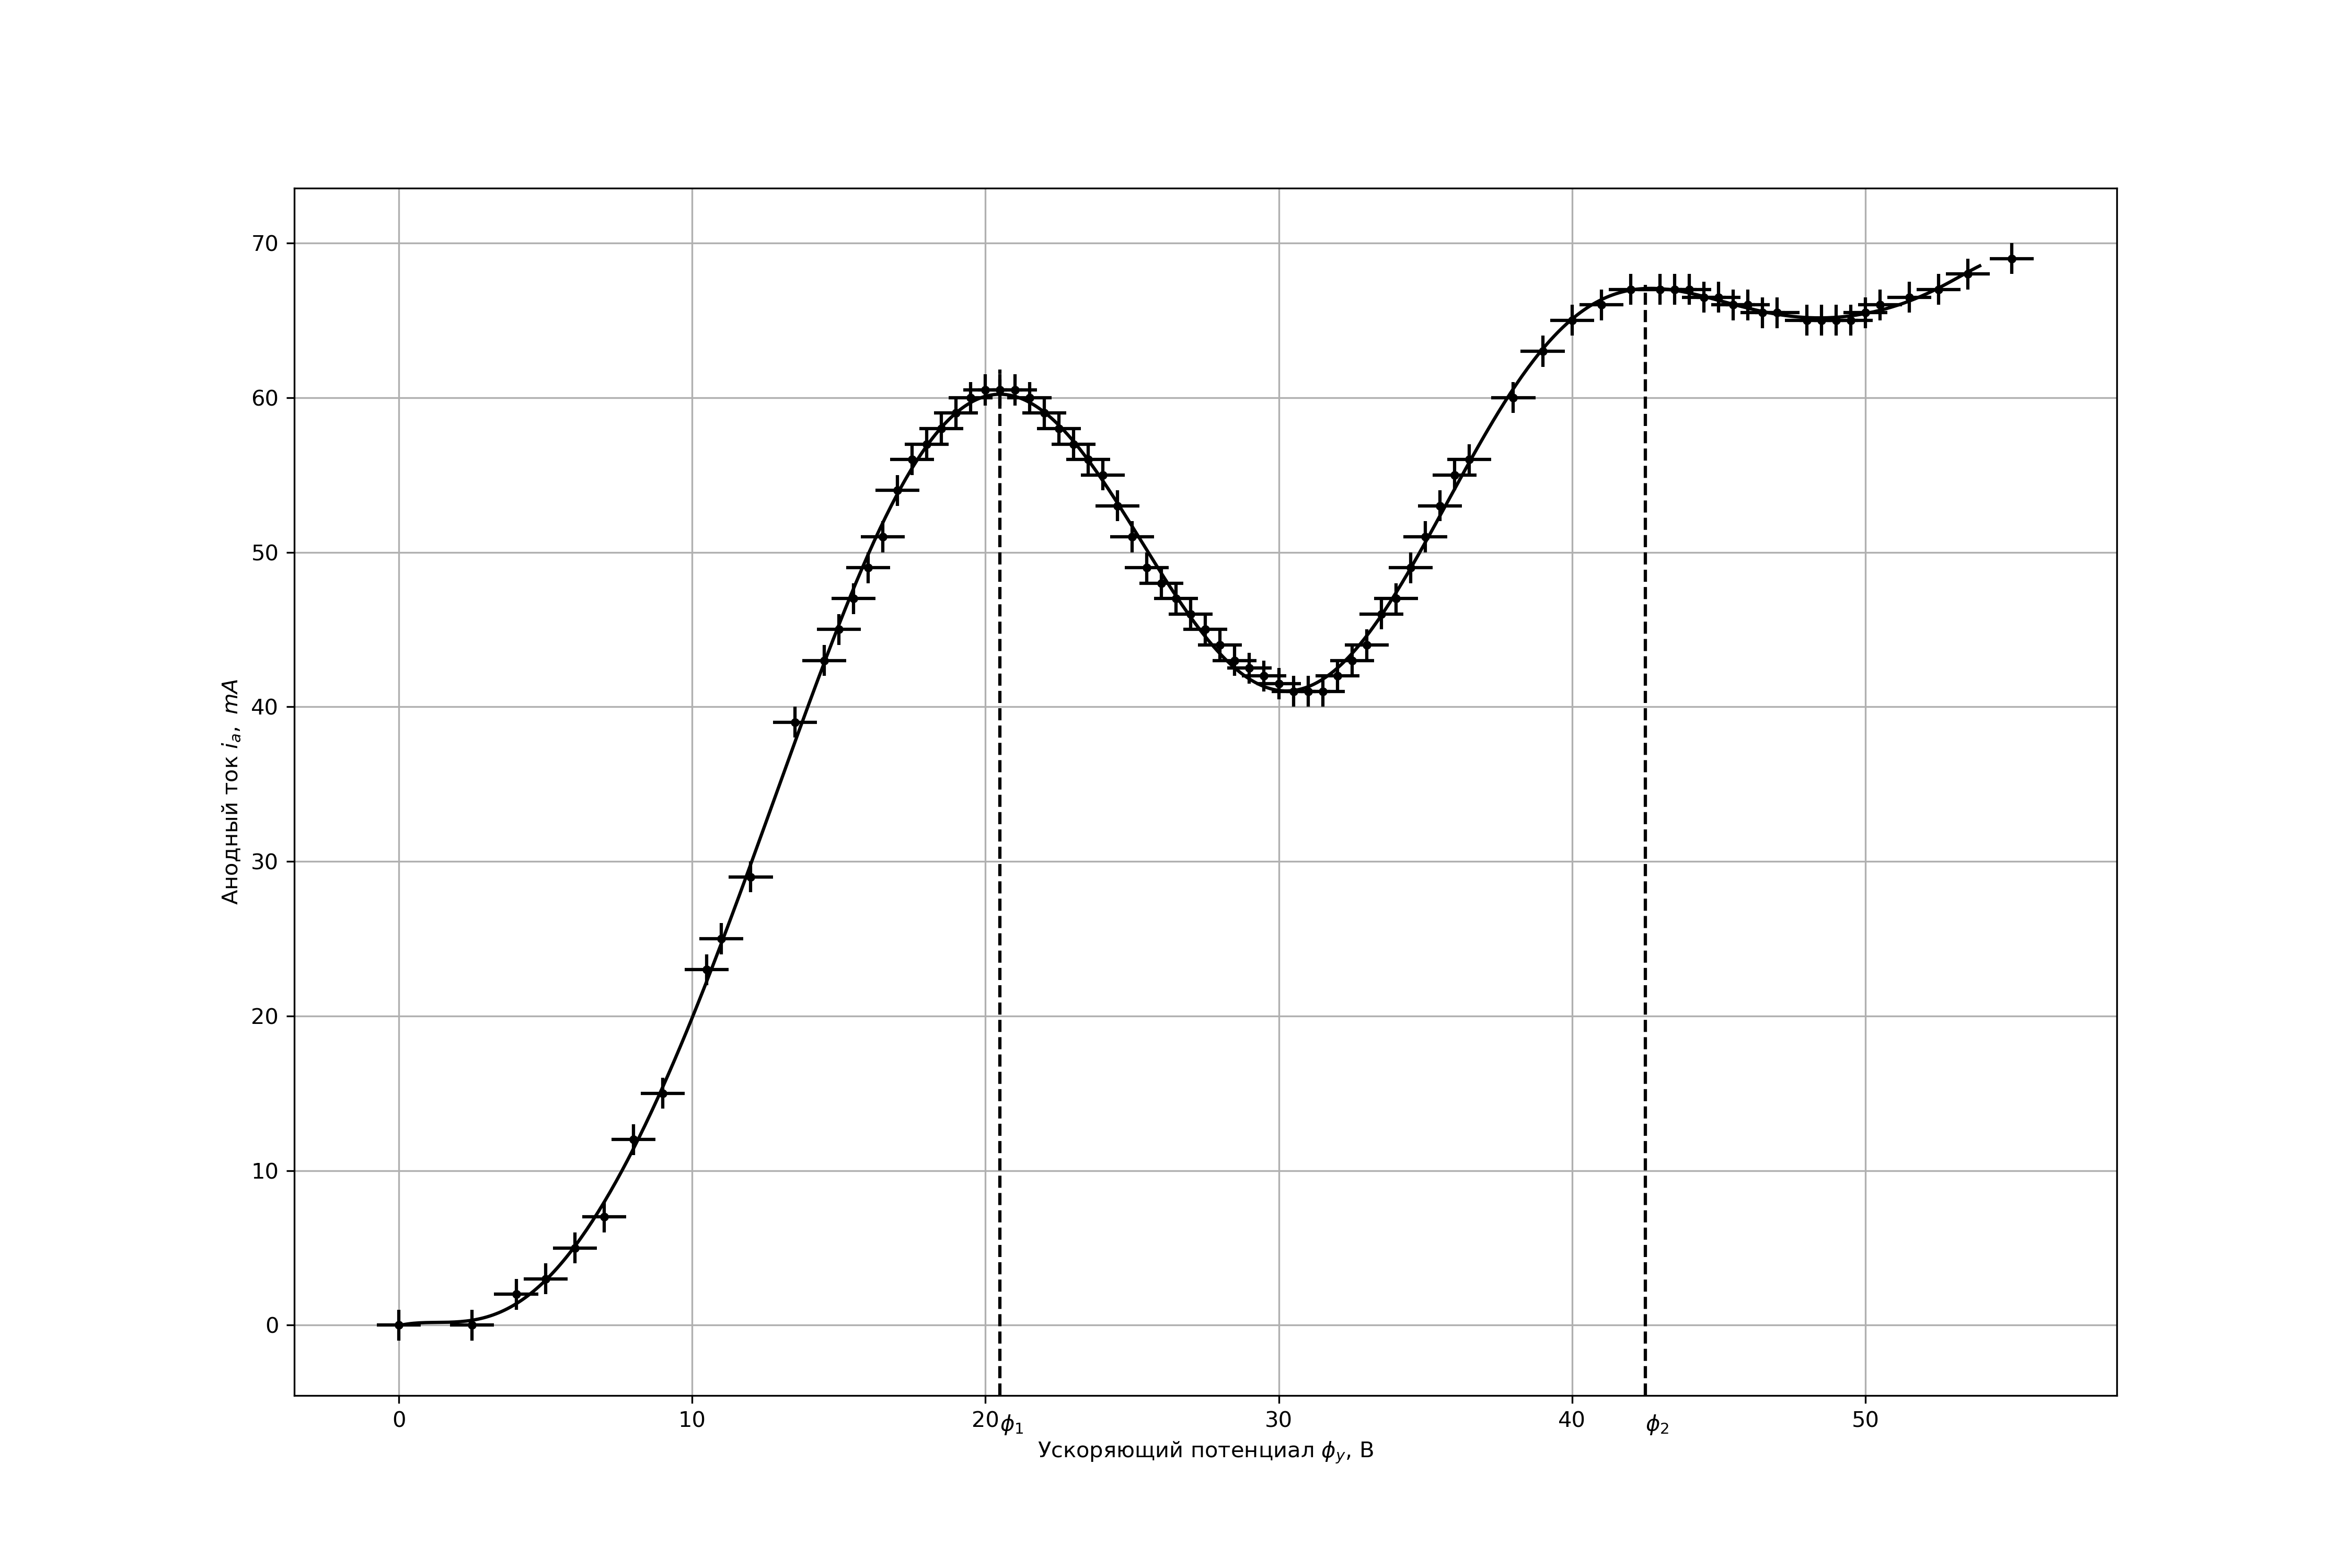
\includegraphics[width=\linewidth]{graphs/1.png}    
\end{minipage}

Резонансный потенциал $\varphi_1=20.5\pm 0.75$ Эв

Потенциал $\varphi_2=42.5 \pm 0.75$ Эв

Разность энергитических уровней $E_1-E_0=e\varphi_1=20.5\pm 0.75$ Эв

Табличное значение $E_1-E_0=21.2$ Эв
\subsection{Определение ионизационного потенциала}
 При разных значениях запирающего потенциала, превышающего потенциал ускорения, была снята зависимость анодного тока от
  ускоряющего потенциала. 

\begin{minipage}{\linewidth}
    \centering
    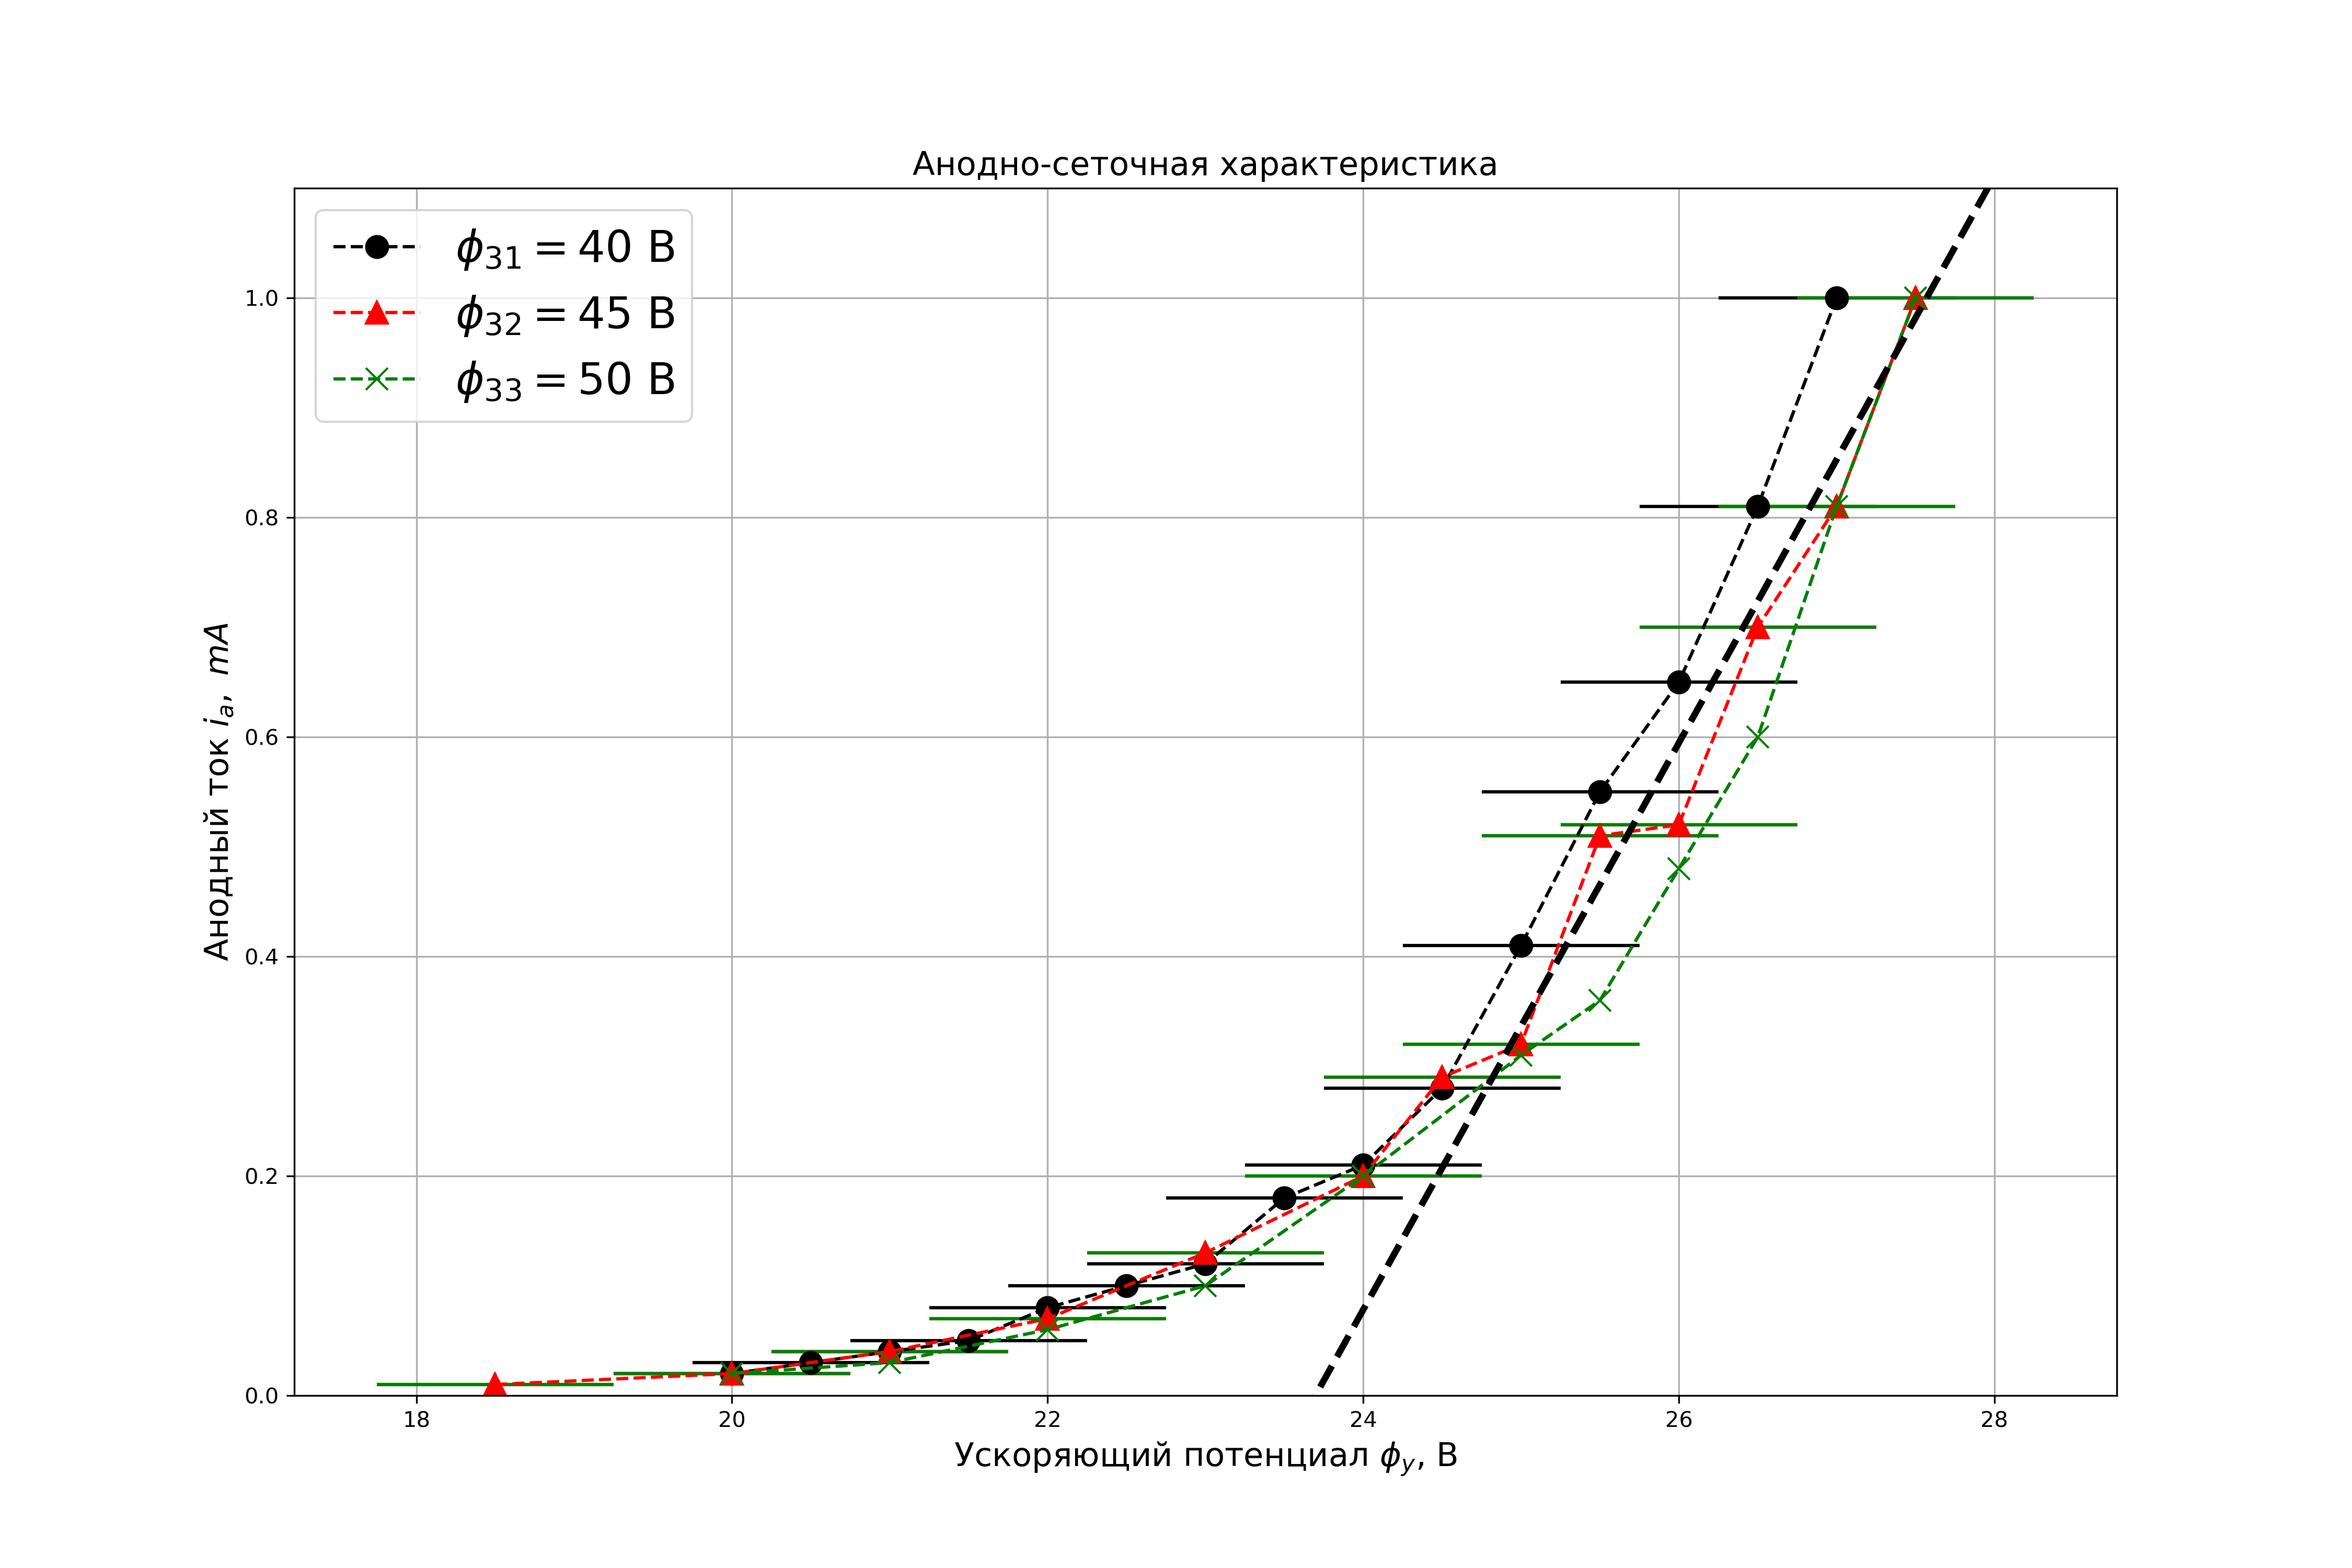
\includegraphics[width=\linewidth]{graphs/2.png}    
\end{minipage}

Потенциал ионизации $\varphi_u$ определялся как значительное увеличение анодного тока при повышении ускоряющего
потенциала. При значениях, близких, но меньше $\varphi_u$ анодный ток может появляться ввиду разброса электронов по
скоростям при эмитировании с катода. Электроны, обладающие большей начальной скоростью могут ионизировать атом, при том
что большая часть атомов останется не ионизированными. Определенный $\varphi_u$ составил $\varphi_u=23.7\ \text{Эв}$ 

Для ионизации атомов газа необходимо, чтобы энергия, которую приобретает электрон на длине свободного пробега $\Delta W_{\lambda}=e\lambda \displaystyle\dv{\varphi}{n}$
была бы не меньше энергии $E_u-E_1=e(\varphi_u-\varphi_1)=3.2\text{ Эв}.$ 


\section{Вывод}
В проведенной работе был экспериментально подтвержден вид сеточной характеристики и ионного тока. Были получены значения
$\varphi_1$, $\varphi_2$ и $\varphi_u$, напрямую связанные со свойствами исследуемого газа.
\end{document}